\section{Widman ``holes filling technique''}

A sharp version of the Caccioppoli-Leray inequality~\eqref{CLI} has been proven by \underline{Widman}.\\
We can illustrate that in the simple case of \(f=0, F=0\).\\
Observe that, with the notation of the~\eqref{CLI} proof, since \(\abs{\nabla u}\leq \frac{4}{R} \chi_{B_{R}\setminus B_{\sfrac{R}{2}}}\) one obtains
\begin{gather}
    \int\limits_{B_{\sfrac{R}{2}}}^{} \abs{\nabla u(x)}^{2} \dd{x} leq \frac{c}{R^{2}} \int\limits_{B_{R} \setminus B_{\sfrac{R}{2}}}^{} \abs{u(x)-k}^{2} \dd{x} \label{001}
\end{gather}
for some positive constant \(c\) independent of \(R\).\\
Now the idea is to choose \(\kappa := \fint_{B_{R}\setminus B_{\sfrac{R}{2}}} u(x) \dd{x}\) so that we can estimate the r.h.s of~\eqref{001} using the Poincarè inequality with explicit scaling, i.e.
\begin{gather}
    \int\limits_{B_{R}\setminus B_{\sfrac{R}{2}}}^{} \abs{u(x)-\fint\limits_{B_{R}\setminus B_{\sfrac{R}{2}}}^{} u \dd{x} }^{2} \dd{x} \leq cR^{2}\int\limits_{B_{R}\setminus B_{\sfrac{R}{2}}}^{} \abs{\nabla u(x)}^{2} \dd{x}
\end{gather}
to get
\begin{align}
                           & \int\limits_{B_{\sfrac{R}{2}}}^{} \abs{\nabla u(x)}^{2} \dd{x} \leq c \int\limits_{B_{R}\setminus B_{\sfrac{R}{2}}}^{} \abs{\nabla u(x)}^{2} \dd{x} \\
    \Leftrightarrow  (c+1) & \int\limits_{B_{\sfrac{R}{2}}}^{} \abs{\nabla u(x)}^{2} \dd{x} \leq c \int\limits_{B_{R}}^{} \abs{\nabla u(x)}^{2} \dd{x}
\end{align}
Setting \( \vartheta := \frac{c}{c+1}<1\) we get
\begin{gather}
    \int\limits_{B_{\sfrac{R}{2}}}^{} \abs{\nabla u(x)}^{2} \dd{x} \leq \vartheta \int\limits_{B_{R}}^{} \abs{\nabla u(x)}^{2} \dd{x}
\end{gather}
\underline{Iterating} the previous estimates \(d\) times for radii
\begin{gather}
    2^{1}r \to 2^{2}r \to 2^{3}r \to \dots \to 2^{d}r
\end{gather}
and choosing \(r\) such that
\begin{gather}
    2^{d}r < R< 2^{d+1}r \label{002}
\end{gather}
we get
\begin{gather}
    \int\limits_{B_{R}}^{} \abs{\nabla u}^{2} \dd{x} \leq \vartheta^{d}\int\limits_{B_{R}}^{} \abs{\nabla u}^{2} \dd{x}
\end{gather}
Setting \(\alpha \log_{2}(\sfrac{1}{\vartheta})\), i.e. \(\vartheta = \sfrac{1}{2^{\alpha}}\) we have
\begin{gather}
    \vartheta^{d}= \frac{1}{2^{\alpha d}} = {\Big( \frac{1}{2^{d}} \Big)}^{\alpha} \overset{\eqref{002}}{\leq} 2^{\alpha}{\Big( \frac{r}{R} \Big)}^{\alpha}.
\end{gather}
Hence,
\begin{gather}
    \int\limits_{B_{r}}^{} \abs{\nabla u}^{2} \dd{x} \leq 2^{\alpha} {\Big( \frac{r}{R} \Big)}^{\alpha} \int\limits_{B_{R}}^{} \abs{\nabla u}^{2} \dd{x}.
\end{gather}
For \(n=2\) the estimate above implies \(u \in C^{0, \sfrac{\alpha}{2}}(\Omega; \mathbb{R}^{m})\).\\
In fact the idea that the decay of the \(L^{p}\)-norm of the gradient is related to its Hölder continuity will play a crucial role in the rest of the course, and we will discuss in detail in the next lectures.

\section{Continuity via embedding}

The Sobolev embedding theorem for \(W^{1,p}(\Omega; \mathbb{R})\) says that
\begin{align}
    \begin{cases}
        p<n \qquad   & W^{1,p}(\Omega; \mathbb{R}) \hookrightarrow L^{p^{\star}}(\Omega;\mathbb{R}) \quad \text{continuously} \quad p^{\star}=\frac{np}{n-p} \\
        p=n \qquad   & W^{1,n}(\Omega; \mathbb{R}) \hookrightarrow L^{q^{\star}}(\Omega;\mathbb{R}) \quad \text{compactly} \quad \forall 1 \leq q < \infty   \\
        p > n \qquad & W^{1,p}(\Omega; \mathbb{R}) \hookrightarrow C^{0, 1-\sfrac{n}{p}}(\Omega;\mathbb{R}) \quad \text{continuously}
    \end{cases}
\end{align}
Hence a way to prove continuity of a Sobolev function is to prove that it belongs to \(W^{1,p}\) for \(p>n\).

\section{Embedding for higher order Sobolev spaces}

We recall that higher order Sobolev spaces \(W^{k,p}(\Omega; \mathbb{R})\) with \(k \geq 1\) integer and \(1 \leq p \leq \infty \) are recursively defined as
\begin{gather}
    W^{k,p}(\Omega, \mathbb{R}):= \{ u \in W^{1,p}(\Omega; \mathbb{R}): \nabla u \in W^{k-1,p}(\Omega; \mathbb{R}^{n})\}.
\end{gather}
Another way to prove continuity, applicable if \(p < n\), is to use \(W^{k,p}\) for \(k\) large enough. In fact, it holds true that:
\begin{enumerate}[label= (\arabic*)]
    \item if \(kp<n\) then \(W^{k,p}(\Omega; \mathbb{R})\hookrightarrow L^{p}(\Omega;\mathbb{R})\) for all \(1 \leq q \leq p_{k}^{\star}\), when \(p_{k}^{\star}=\frac{np}{n-kp}\)
    \item if \(kp=n\) then \(W^{k,p}(\Omega; \mathbb{R}) \hookrightarrow L^{q}(\Omega; \mathbb{R}) \) for all \( 1 \leq q\leq \infty \)
    \item if \( kp > n \) and \( k-\frac{n}{p}\notin \mathbb{N}, W^{k,p}(\Omega;\mathbb{R}) \hookrightarrow C^{l,\alpha}(\overline{\Omega; \mathbb{R}})\) for \( l= \left\lfloor k-\frac{n}{p} \right\rfloor  \) and \( 0 \leq \alpha\leq k-\frac{n}{p}-l \)
    \item if \( kp> n \) and \( k-\frac{n}{p}=l+1 \in \mathbb{N}, W^{k,p}(\Omega; \mathbb{R}) \hookrightarrow C^{l,\alpha} (\overline{\Omega}; \mathbb{R})\) for all \( 0 \leq \alpha < 1 \)
\end{enumerate}

\section{A priori estimates and the Nirenberg method}

If \( u \in  H_{loc}^{1} (\Omega; \mathbb{R})  \) (for the moment we are not interested at the behavior of \( u \) at \( \partial \Omega \)) is a weak solution of a system of elliptic PDEs we cannot apply previous remark to prove classical regularity, i.e.\ differentiability of \( u \) without assuming existence and some integrability of higher order weak derivatives of \( u \). In fact the previous remark is not really exploiting the equation.\\
\par
\underline{How to gain better integrability?}\\
What   follows goes under the name of \underline{Nirenberg's method}.\\
Let us consider the simplest setting and consider a solution \( u \in H_{loc}^{1} (\Omega)  \) of the Poisson equation
\begin{gather}
    - \Delta u = f, \qquad f \in L_{loc}^{2} (\Omega ;\mathbb{R})
\end{gather}
We want to prove that \( u \in H_{loc}^{2} (\Omega ; \mathbb{R}) =W_{loc}^{2,2} (\Omega ;\mathbb{R})  \), as this will be the first step to transfer regularity information from the data \( f \) to the solution \( u \).\\
\\
Let us start with supposing that we already knew that \( \partial_{x_{\alpha }} u \in H_{loc}^{1} (\Omega ;\mathbb{R})  \), then we know that
\begin{gather}
    -\Delta (\partial_{x_{\alpha }} u) = \partial_{x_{\alpha }} f \qquad \text{in a weak sense}
\end{gather}
To check it, test \( -\Delta u=f \) with \( \partial_{x_{\alpha }} \phi  \) and integrate by parts to get
\begin{align}
    \int \nabla u \nabla (\partial_{x_{\alpha }}\phi )  \dd{x}           & = \int f \partial_{x_{\alpha }}\phi  \dd{x}                                                                                                                                                       \\
    \overset{=}{\int \nabla \partial_{x_{\alpha }}(\nabla \phi)  \dd{x}} & \overset{I.P.}{=} - \int \underbrace{\partial_{x_{\alpha }} \Delta u}_{\Delta (\partial_{x_{\alpha }} u) } \cdot \Delta \phi \dd{x} = - \int \Delta (\partial_{x_{\alpha }}u) \Delta \phi  \dd{x}
\end{align}
Weak derivatives commute:
\begin{gather}
    \int \partial_{1}\partial_{2} u \phi  \dd{x} \overset{I.P.}{=} \int u \partial_{1} \partial_{2} \phi  \dd{x} \overset{\phi \text{ is regular}}{=} \int u \partial_{2}\partial_{1} \phi \dd{x} \overset{I.P.}{=} \int \partial_{2}\partial_{1}u \phi \dd{x}
\end{gather}
Hence \( \int \nabla (\partial_{x_{\alpha }}u) \nabla \phi  \dd{x} = -\int f \partial_{x_{\alpha }}\phi  \dd{x} \) or \( -\nabla (\partial_{x_{\alpha }}u) = \partial_{x_{\alpha}}f \).\\
Hence, for every ball \( B_{R} (x_{0}) \ssubset \Omega  \) (\( \overline{B_{R} (x_{0})} \subset \Omega  \)) we use the Caccioppoli-Leray inequality~\eqref{CLI}  to get:
\begin{gather}
    C_{CL} \int\limits_{B_{\sfrac{R}{2}}(x_{0})}^{} \abs{\nabla (\partial_{x_{\alpha }}u) }^{2} \dd{x} \leq \frac{1}{R^{2}} \int\limits_{B_{R}(x_{0})}^{} \abs{\partial_{x_{\alpha }}U(x) }^{2} \dd{x} + R^{2} \int\limits_{B_{R}(x_{0})}^{} \abs{f(x) }^{2} \dd{x} \qquad \text{\eqref{CLI}}
\end{gather}
that provides an explicit bound on the \( H_{loc}^{2} \) norm of \( u \) in terms of its \( H^{1} \) norm.\\
\par
In the previous discussion we have considered \( u \in H_{loc^{1}}(\Omega ; \mathbb{R})  \) to be a solution of the Poisson equation \( -\nabla u = f \) in \( \Omega  \) with \( f \in L^{2}(\Omega ) \). Assuming \( u\in H_{loc}^{2} \) we have obtained the following Caccioppoli-Leray estimate:
\begin{gather}
    C_{CL} \int\limits_{B_{\sfrac{R}{2}}(x_{0})}^{} \abs{\nabla (\partial_{x_{\alpha }}u) }^{2} \dd{x} \leq \frac{1}{R^{2}} \int\limits_{B_{R}(x_{0})}^{} \abs{\partial_{x_{\alpha }}U(x) }^{2} \dd{x} + R^{2} \int\limits_{B_{R}(x_{0})}^{} \abs{f(x) }^{2} \dd{x} \qquad \text{\eqref{CLI}}
\end{gather}
Can we remove the \enquote{a priori} regularity assumption?\\
Here, for the Poisson equation, it is simple.\\
Consider the convolution \( u \ast \rho_{\epsilon } \). Since \( -\Delta  u = f \) we have \( -\Delta  (u \ast \rho_{\epsilon }) = f\ast \rho _{\epsilon }\).\\
Now observe that
\begin{align}
    C_{CL} \int\limits_{B_{\sfrac{R}{2}}}^{} \abs{\nabla (\partial_{x_{\alpha }}u\ast \rho _{\epsilon })}*2 \dd{x} & \leq \frac{1}{R^{2}}\int\limits_{B_{R}}^{} \abs{\partial_{x_{\alpha }}u \ast \rho _{\epsilon }}^{2} \dd{x} + R^{2}\int\limits_{B_{R}}^{} \abs{f\ast \rho _{\epsilon }}^{2} \dd{x} \\
                                                                                                                   & \leq  \frac{1}{R^{2}} \int\limits_{B_{R}}^{} \abs{\partial_{x_{\alpha }}u}^{2} \dd{x} + R^{2} \int\limits_{B_{R}}^{} \abs{f}^{2} \dd{x}
\end{align}
As a result \( \forall \alpha ,\beta \, \norm{\partial_{x_{\alpha }}\partial_{x_{\beta}}(u\ast \rho _{\epsilon })}_{L_{loc}^{2}} \leq  C \). This means that, up to subsequences \( \partial_{x_{\alpha }}\partial_{x_{\beta}}(u\ast \rho _{\epsilon }) \myxrightharpoonup[\epsilon  \to 0]{L^{2}} g\). Since \( \partial_{x_{\alpha }}(u\ast \rho _{\epsilon }) \myxrightarrow[]{L^{2}} \partial_{x_{\alpha }} u \), we have that \( g = \partial_{x_{\alpha }}\partial_{x_{\beta}}u\) and that the whole sequence \( \partial_{x_{\alpha }}\partial_{x_{\beta}}(u\ast \rho _{\epsilon }) \) converges to \( \partial_{x_{\alpha }}\partial_{x_{\beta}}u \). \\
As a result \( \norm{\partial_{x_{\alpha }}\partial_{x_{\beta}}u}_{L_{loc}^{2}} \leq  C \) and \( u \in H_{loc}^{2} (\Omega )  \).\\
\par

We have used the following result:
\begin{lem}[Stability of weak derivatives]
    \( u_{k}\in W^{1,p}(\Omega )\) for some \( 1 < p < \infty, \forall k \in  \mathbb{N} \). Assume \( u_{k} \myxrightarrow[]{} u  \) in \( L^{p} \) and \( \sup_{k}\norm{\nabla u_{k}}_{p}\leq C \), then \( u\in W^{1,p}(\Omega ) \) and \( \nabla u_{k \myxrightharpoonup[]{}\nabla u} \) in \( L^{p} \).
\end{lem}
The same idea does not work so easily when the coefficients \( A_{ij}^{\alpha \beta } \) are not constant. In fact in this case differentiating the equation produces \enquote{extra terms}.\\
Nirenberg's idea is to use difference quotients instead of derivatives. We introduce the notation
\begin{gather}
    \Delta _{h, \alpha }u(x) = \frac{u(x+he_{\alpha})-u(x)}{h} =: \frac{\tau _{h, \alpha }U(x)-u(x) }{h }
\end{gather}
The following properties can be checked to hold true:
\begin{enumerate}[label= \( \bullet \)  ]
    \item Discrete Leibniz rule
          \begin{align}
              \Delta _{h, \alpha }(uv)
               & = (\tau _{h, \alpha } u) \Delta _{h,\alpha }v + (\Delta _{h, \alpha} u) v    \\
               & =    (\tau _{h, \alpha } v) \Delta _{h,\alpha }u + (\Delta _{h, \alpha} v) u
          \end{align}

    \item Integration by parts rule
          \begin{gather}
              \int\limits_{\Omega}^{} \phi (x) \Delta _{h, \alpha } u(x)   \dd{x} = -\int\limits_{\Omega}^{} u(x) \Delta _{-h, \alpha }\phi (x)    \dd{x}
          \end{gather}
          for all \( \phi \in  C_{c}^{1} (\Omega ; \mathbb{R}), \abs{h}< \operatorname{dist}(\operatorname{spt} \phi, \partial \Omega )  \)
\end{enumerate}
The following lemma provides a characterization of \( W^{1,p} \) functions with \( p>1 \), in terms of uniform \( L^{p} \) bounds of the corresponding discrete partial derivatives.

\begin{lem}[]\label{lemma01}
    Consider \( u\in L_{loc}^{p}(\Omega ;\mathbb{R}) \), with \( 1< p \leq  \infty  \) and fix \( \alpha \in \{ 1,2,\ldots,n \} \). The partial derivative \( \partial_{x_{\alpha }}u \) belongs to \( L_{loc}^{p}(\Omega ;\mathbb{R}) \) if and only if the family \( \Delta _{h,\alpha }u \) is uniformly bounded in \( L_{loc}^{p} \) as \( h \to 0 \).\\
    More precisely, if \( \forall \Omega' \ssubset \Omega \, \exists C=C(\Omega') \) such that
    \begin{gather}
        \abs{\int\limits_{\Omega'}^{} (\Delta _{h,\alpha }u) \phi  \dd{x}}\leq c\norm{\phi }_{L^{p'}(\Omega';\mathbb{R})} \qquad \phi \in C_{c}^{1}(\Omega';\mathbb{R})
    \end{gather}
    with \( \frac{1}{p}+\frac{1}{p'}=1 \) and \( \abs{h}< \frac{1}{2} \operatorname{dist}(\Omega';\partial \Omega )  \).
\end{lem}
We now see how the previous lemma allows us to obtain regularity. We stick to the Poisson equation for the moment. \par
Suppose \( f \in H_{loc}^{1}(\Omega ;\mathbb{R})  \) and \( -\Delta u=f \) for some \( u \in H_{loc}^{1}(\Omega ; \mathbb{R})  \).\\
Being the equation translation invariant, we can write \( -\Delta (\tau _{h,\alpha }u) = \tau _{h, \alpha }f \), hence \( -\Delta (\Delta _{h, \alpha }u) = \Delta _{h, \alpha }f \) for any \( \Omega' \ssubset \Omega  \) and \( \abs{h}< \operatorname{dist}(\Omega', \partial \Omega )  \). \\
By Lemma~\ref{lemma01} it holds \( \Delta _{h, \alpha }f \) is bounded in \( L_{loc}^{2} \) uniformly in \( h \). By~\eqref{CLI} \( \abs{\nabla \Delta _{h, \alpha }U} \) is bounded in \( L_{loc}^{2}(\Omega ;\mathbb{R})  \), thanks to the Lemma~\ref{lemma01} (applied componentwise) we have that
\begin{gather}
    \partial_{x_{\alpha }}(\nabla u) \in L_{loc}^{2}(\Omega ;\mathbb{R}^{n})
\end{gather}

That is, by the arbitrariness of \( \alpha \in \{ 1,2,\ldots,n \} \), \( u \in H_{loc}^{2}(\Omega ;\mathbb{R})  \). We are left to prove Lemma~\ref{lemma01}.\\
\par
We now state and prove the first interior regularity theorem.

\begin{thm}[\(H^{2}\)-regularity]
    Let \( \Omega  \) be an open domain in \( \mathbb{R} \). Consider a map \( A\in C_{loc}^{0,1}(\Omega ; \mathbb{R}^{m^{2}\times n^{2}})  \)
    such that \( A(x) := A_{ij}^{\alpha \beta }(x)\) satisfies the Legendre-Hademard condition~\eqref{LH} for some continuous and positive ellipticity function \( \lambda : \Omega \to \mathbb{R}\),
    as well as the uniform bound
    \[ \sup_{x \in \Omega } \abs{A_{ij}^{\alpha \beta }(x)}\leq \Lambda < \infty. \] Then,
    for every \( u \in H_{loc}^{1}(\Omega ; \mathbb{R}^{m})  \) weak solution of the equation \[ - \sum\limits_{\alpha ,\beta ,j}^{}\partial_{x_{\alpha }}(A_{ij}^{\alpha \beta }\partial_{x_{\beta}}u^{j}) = f_{i}-\sum\limits_{\alpha}^{} \partial_{x_{\alpha }}F_{i}^{\alpha } \qquad i=1,2,\ldots,m  \]
    with data \( f \in L_{loc}^{2}(\Omega ;\mathbb{R}^{m}) \) and \( F \in H_{loc}^{1}(\Omega ;\mathbb{R}^{m \times n})  \), one  has that \( u \in H_{loc}^{2}(\Omega ; \mathbb{R}^{m})  \) and for every \( \Omega' \ssubset \Omega'' \ssubset \Omega \) there exists \( c:=c(\Omega', \Omega'', A)  \) such that
    \[ \int\limits_{\Omega'}^{} \abs{\nabla ^{2}u}^{2} \dd{x} \leq c \left( \int\limits_{\Omega''}^{} \abs{u}^{2} \dd{x} + \int\limits_{\Omega''}^{} \abs{f}^{2} \dd{x} + \int\limits_{\Omega''}^{} \abs{\nabla F}^{2} \dd{x} \right) \]
\end{thm}

\begin{remark}[]
    Even if we have stated the theorem for a generic \( \Omega' \ssubset \Omega  \), it is enough to prove it for balls inside \( \Omega  \).
    More precisely. It is enough to prove it for balls \( B_{R}(x_{0}) \) where \( x_{0}\in \Omega' \) and \( R < \frac{1}{2}\overset{dist}(\Omega', \partial \Omega )  \).
    \begin{center}
        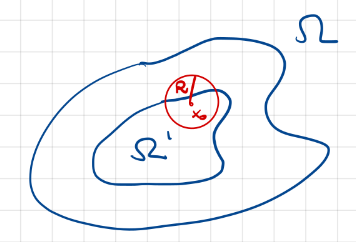
\includegraphics[scale=0.45]{pictures/picture02.png}
    \end{center}
    The general result can then be obtained by a compactness and covering argument (Exercise).\\
    For the case of a ball we need to prove that
    \[ \int\limits_{B_{\sfrac{R}{2}(x_{0}) }}^{} \abs{\nabla ^{2}u}^{2} \dd{x} \leq c \left( \int\limits_{B_{2R}(x_{0})}^{} \abs{u}^{2} \dd{x} + \int\limits_{B_{2R}(x_{0})}^{} \abs{f}^{2} \dd{x} + \int\limits_{B_{2R}(x_{0})}^{} \abs{\nabla F}^{2} \dd{x} \right) \] for every \( x_{0} \in \Omega' \).
\end{remark}